\documentclass[accentcolor=tud2c,usenames,dvipsnames,colorbacktitle,inverttitle,landscape,german,presentation,t]{tudbeamer}
\usepackage[english]{babel}
\usepackage{amsmath}
\usepackage{amssymb}
\usepackage{slashed}
\usepackage{color}
\usepackage{physics}
\usepackage{graphicx}
\usepackage{braket}
% \usepackage[utf8]{inputenc}

\begin{document}

  \newcommand{\U}[1]{\textrm{U}(#1)}
\newcommand{\suthree}{\textrm{SU}(3)}
\newcommand{\suxsu}{\suthree_{L} \times \suthree_{R}}
\newcommand{\suxsuxu}{\suxsu \times \U{1}_V}
\newcommand{\suxsuxuxu}{\suxsu \times \U{1}_L \times \U{1}_R}
\newcommand{\uxu}{\U{3} \times \U{3}}
\newcommand{\sul}{\textrm{SU}(3)_{L}}
\newcommand{\sur}{\textrm{SU}(3)_{R}}
\newcommand{\Phidag}{\Phi^{\dagger}}
\newcommand{\Phistar}{\Phi^{*}}
\newcommand{\dmulo}[1]{\partial_{\mu}#1}
\newcommand{\dmuhi}[1]{\partial^{\mu}#1}
\newcommand{\dmulop}[1]{(\partial_{\mu}#1)}
\newcommand{\dmuhip}[1]{(\partial^{\mu}#1)}
\newcommand{\dmulox}[2]{\partial_{\mu}^{#2}#1}
\newcommand{\dmuhix}[2]{\partial^{\mu}^{#2}#1}
\newcommand{\dmulopx}[2]{(\partial_{\mu}^{#2}#1)}
\newcommand{\dmuhipx}[2]{(\partial^{\mu}^{#2}#1)}
\newcommand{\Gmu}{G^{\mu}}
\newcommand{\Jmu}{J^{\mu}}
\newcommand{\timeorder}[1]{T[#1]}
% \newcommand{\4ddelta}[2]{\delta^{4}(#1 - #2)}
\newcommand{\vecoct}{V_{a}^{\mu}}
\newcommand{\axvoct}{A_{a}^{\mu}}
\newcommand{\vecsing}{V^{\mu}}
\newcommand{\axvsing}{A^{\mu}}
\newcommand{\vecoctexpl}{\bar{q}\gamma^{\mu}\frac{\lambda_a}{2}q}
\newcommand{\axvoctexpl}{\bar{q}\gamma^{\mu}\gamma_5\frac{\lambda_a}{2}q}
\newcommand{\vecsingexpl}{\bar{q}\gamma^{\mu}q}
\newcommand{\axvsingexpl}{\bar{q}\gamma^{\mu}\gamma_5q}
\newcommand{\scalardensity}[1]{S_{#1}}
\newcommand{\scalardensityx}[2]{\scalardensity{#1}(#2)}
\newcommand{\scalardensityexpl}[1]{\bar{q} \lambda_{#1} q}
\newcommand{\scalardensityexplx}[2]{\bar{q}(#2) \lambda_{#1} q(#2)}
\newcommand{\pscalardensity}[1]{P_{#1}}
\newcommand{\pscalardensityx}[2]{\pscalardensity{#1}(#2)}
\newcommand{\pscalardensityexpl}[1]{i \bar{q} \gamma_5 \lambda_{#1} q}
\newcommand{\pscalardensityexplx}[2]{i \bar{q}(#2) \gamma_5 \lambda_{#1} q(#2)}
% \newcommand{\commutator}[2]{[#1, #2]}
\newcommand{\lext}{\mathcal{L}_{\textrm{ext}}}


  \setbeamerfont{footline}{size=\fontsize{1}{1}\selectfont}

  \title{Chiral Green's functions and Ward identities}
  \subtitle{\small{Matthias Heinz}}
  \author{Matthias Heinz}
  \institute[Institut f\"ur Kernphysik, TU Darmstadt]{Institut f\"ur Kernphysik, TU Darmstadt}
  \date{January 30, 2020}

  \setbeamertemplate{section in toc}[ball unnumbered]
  \setbeamertemplate{subsection in toc}[ball unnumbered]

  \nocite{*}

  \begin{titleframe}
    \vskip3em
    \begin{columns}[c]
      \begin{column}{0.8\textwidth}
        Outline:
          \vskip2em
        \begin{enumerate}
          \item Ward identities in a $\U{1}$ example
          \vskip2em
          \item Chiral Ward identities via the algebra of currents
          \vskip2em
          \item The chiral generating functional
        \end{enumerate}
      \end{column}
    \end{columns}
      % 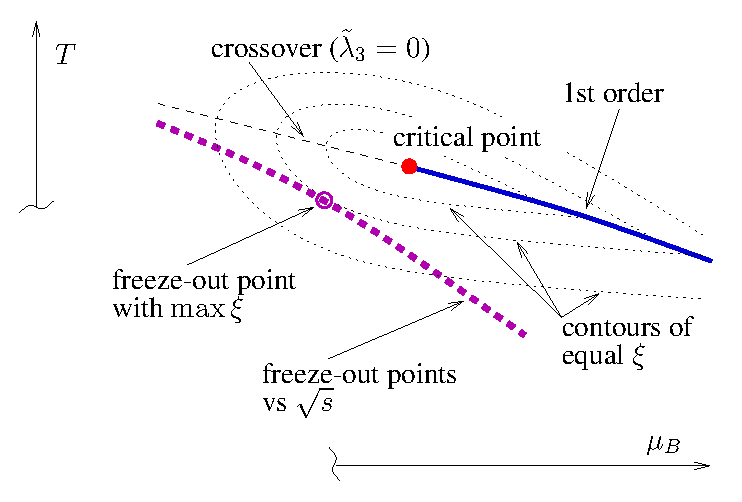
\includegraphics[width=0.75\textwidth]{figures/05/critical_point_illustration}
      % \\\footnotesize{Stephanov 2009}
  \end{titleframe}

  \section{Ward identities in a $\U{1}$ example}

  \begin{frame}
    \frametitle{Scalar $\Phi^4$ theory with a global $\U{1}$ symmetry}
    \begin{equation*}
      \mathcal{L}^0 = \frac{1}{2}(\dmulop{\Phidag}\dmuhip{\Phi})
      - \frac{m^2}{2} \Phidag \Phi - \frac{\lambda}{4} (\Phidag \Phi)^2
    \end{equation*}

    \vskip3em

    \begin{columns}[c]
      \begin{column}{0.8\textwidth}
        Global $\U{1}$ symmetry:

        \begin{equation*}
        \begin{array}{cc}
          \Phi \rightarrow (1 + i \epsilon) \Phi, &
          \Phidag \rightarrow (1 - i \epsilon) \Phidag, \\
        \end{array}
        \end{equation*}

        \vskip1em

        Conserved Noether current:

        \begin{equation*}
          \Jmu = i (\dmuhip{\Phidag} \Phi - \Phidag \dmuhip{\Phi})
        \end{equation*}
      \end{column}
    \end{columns}
  \end{frame}

  \begin{frame}
    \frametitle{Scalar $\Phi^4$ theory with a global $\U{1}$ symmetry}

    \begin{columns}[c]
      \begin{column}{0.8\textwidth}
        Example Green's function:

        \begin{equation*}
          \Gmu(x,y,z) = \mel*{0}{\timeorder{\Phi(x)\Jmu(y)\Phidag(z)}}{0},
        \end{equation*}

        \vskip1em

        Symmetry constraint:

        \begin{equation*}
          \begin{array}{cc}
            \Jmu \rightarrow \Jmu, &
            \Gmu \rightarrow \Gmu, \\
          \end{array}
        \end{equation*}

        \vskip1em

        Example Ward identity:

        \begin{align*}
          \dmulox{\Gmu(x,y,z)}{y} = & (\delta^4(y-x) - \delta^4(y-z))\mel*{0}{\timeorder{\Phi(x) \Phidag(z)}}{0} \\
                                    & + \mel*{0}{\timeorder{\Phi(x) \dmulopx{\Jmu(y)}{y} \Phidag(z)}}{0},
        \end{align*}
      \end{column}
    \end{columns}
  \end{frame}

  % \begin{frame}
  %   \frametitle{Recap of path integral formalism \\ Maybe just skip and explain on actual generating functional}
  %   \begin{columns}[c]
  %     \begin{column}{0.8\textwidth}
  %       Green's functions via path integral:
  %
  %       \begin{equation*}
  %         \mel{0}{\timeorder{\Phidag(x) \Phi(y)}}{0} =
  %         \int \mathcal{D}\Phistar \mathcal{D}\Phi \Phistar(x) \Phi(y) \exp(i S[\Phi, \Phistar]),
  %       \end{equation*}
  %
  %       Generating functional:
  %
  %       \begin{equation*}
  %       W[j, j^{*}] = \mel*{0}{\timeorder{\exp(i\int d^4x[j(x) \Phidag (x) + j^{*}(x) \Phi(x)])}}{0},
  %       \end{equation*}
  %
  %       Green's functions via functional derivatives:
  %
  %       \begin{equation*}
  %         \mel{0}{\timeorder{\Phidag(x) \Phi(y)}}{0} = \left.\left(-i\frac{\delta}{\delta j(x)} \right) \left(-i\frac{\delta}{\delta j^{*}(y)} \right) W[j, j^{*}] \right\rvert_{j=0,j^{*}=0},
  %       \end{equation*}
  %     \end{column}
  %   \end{columns}
  % \end{frame}

  \begin{frame}
    \frametitle{Generating functional for $\Phi^4$}
    \begin{columns}[c]
      \begin{column}{0.8\textwidth}
        Generating functional:
        \begin{equation*}
          W[j, j^{*}, j_{\mu}] = \mel*{0}{\timeorder{\exp{i\int d^4x[j(x) \Phidag (x) + j^{*}(x) \Phi(x) + j_{\mu}(x) \Jmu(x)]}}}{0},
        \end{equation*}
        Our example Green's function:
        \begin{equation*}
          \Gmu(x,y,z) = \left.(-i)^3 \frac{\delta^3 W[j, j^{*}, j_{\mu}]}{\delta j^{*}(x) \delta j_{\mu}(y) \delta j(z)}\right\rvert_{j=0,j^{*}=0,j_{\mu}=0},
        \end{equation*}
        As path integral:
        \vskip-1em
    \begin{equation*}
      \only<1>{W[j, j^{*}, j_{\mu}] = \int \mathcal{D}\Phistar \mathcal{D}\Phi \exp(i \int d^4x[\mathcal{L}^{0}(x) + \mathcal{L}_{\textrm{ext}}(x)]),}
      \only<2>{W[j, j^{*}, j_{\mu}] = \int \mathcal{D}\Phistar \mathcal{D}\Phi \exp(i S[\Phi, \Phistar, j, j^{*}, j_{\mu}]),}
    \end{equation*}
    \only<1>{
      \begin{equation*}
        \mathcal{L}_{\textrm{ext}}(x) = j(x) \Phi^{*} (x) + j^{*}(x) \Phi(x) + j_{\mu}(x) \Jmu(x),
      \end{equation*}
    }
    \only<2>{Note: Only in the presence of external fields can we demand $\mathcal{L}$ remain invariant under \textit{local} transformations.}
      \end{column}
    \end{columns}

  \end{frame}

  \begin{frame}
    \frametitle{The master equation for $\Phi^4$}
    \begin{columns}[c]
      \begin{column}{0.8\textwidth}

    Demanding $S[\Phi, \Phidag, j, j^{*}, j_{\mu}] = S[\Phi^{\prime}, \Phi^{\prime \dagger}, j^{\prime}, j^{\prime*}, j^{\prime}_{\mu}]$ gives:
    \begin{align*}
    j(x) & \rightarrow (1 + i \epsilon(x))j(x), \\
    j^{*}(x) & \rightarrow (1 - i \epsilon(x))j^{*}(x), \\
    j_{\mu}(x) & \rightarrow j_{\mu} - \dmulop{\epsilon(x)},
    \end{align*}
    % \begin{equation*}
    %   \begin{array}{ccc}
    %     j(x) \rightarrow (1 + i \epsilon(x))j(x), &
    %     j^{*}(x) \rightarrow (1 - i \epsilon(x))j^{*}(x), &
    %     j_{\mu}(x) \rightarrow j_{\mu} - \dmulop{\epsilon(x)}, \\
    %   \end{array}
    % \end{equation*}
    We observe that this also means:
    \begin{equation*}
      W[j, j^{*}, j_{\mu}] = W[j^{\prime}, j^{\prime*}, j^{\prime}_{\mu}],
    \end{equation*}
    Master equation:
    \begin{equation*}
      \only<1>{0 = \int d^{4}x \epsilon(x) \left[ i j(x) \frac{\delta}{\delta j(x)} - i j^{*}(x) \frac{\delta}{\delta j^{*}(x)} + \dmulox{\frac{\delta}{\delta j_{\mu}(x)}}{x} \right] W[j, j^{*}, j_{\mu}],}
      \only<2>{0 = \left[ j(x) \frac{\delta}{\delta j(x)} - j^{*}(x) \frac{\delta}{\delta j^{*}(x)} - i \dmulox{\frac{\delta}{\delta j_{\mu}(x)}}{x} \right] W[j, j^{*}, j_{\mu}],}
    \end{equation*}
      \end{column}
    \end{columns}
  \end{frame}

  \begin{frame}
    \frametitle{QCD in the chiral limit}
    \begin{columns}[c]
      \begin{column}{0.8\textwidth}
        \begin{equation*}
\mathcal{L}_{\textrm{QCD}}^{0} = \sum_{l=u,d,s}(\bar{q}_{R,l}i\slashed{D}q_{R,l} + \bar{q}_{L,l}i\slashed{D}q_{L,l})
- \frac{1}{4} \mathcal{G}_{a\mu\nu} \mathcal{G}_{a}^{\mu\nu},
        \end{equation*}

        Symmetry group:
        \begin{equation*}
        \U{3}_{L}\times\U{3}_{R} \xrightarrow[]{\textrm{Quantization}}\suxsuxu
        \end{equation*}
      \end{column}
    \end{columns}

    \vskip3em
    \begin{columns}[t]
      \begin{column}{0.45\textwidth}
        Conserved currents:
        \begin{itemize}
          \item $\vecoct = R_{a}^{\mu} + L_{a}^{\mu} = \vecoctexpl$,
          \item $\axvoct = R_{a}^{\mu} - L_{a}^{\mu} = \axvoctexpl$,
          \item $\vecsing = R^{\mu} + L^{\mu} = \vecsingexpl$,
        \end{itemize}
      \end{column}
      \begin{column}{0.45\textwidth}
        Color-neutral quadratic forms:
        \begin{itemize}
          \item $\scalardensityx{a}{x} = \scalardensityexplx{a}{x}$,
          \item $\pscalardensityx{a}{x} = \pscalardensityexplx{a}{x}$,
        \end{itemize}
        Note: $a=0,...,8$
      \end{column}
    \end{columns}
  \end{frame}

  \begin{frame}
    \frametitle{Chiral Green's functions and Ward identities \\ \small{\textit{An example}}}
    \begin{columns}[c]
      \begin{column}{0.8\textwidth}
      Green's function:
\begin{equation*}
\Gmu_{APab}(x, y) = \mel*{0}{\timeorder{\axvoct(x)\pscalardensityx{b}{y}}}{0},
\end{equation*}

      Ward identity:
      \end{column}
    \end{columns}
    \vskip1em

\begin{equation*}
\dmulox{\Gmu_{APab}(x,y)}{x} = \delta(x_0 - y_0) \mel*{0}{\commutator{A_{a}^{0}(x)}{P_{b}(y)}}{0}
+ \mel*{0}{\timeorder{\dmulopx{\axvoct(x)}{x}\pscalardensityx{b}{y}}}{0},
\end{equation*}

\vskip1em

    \begin{columns}[c]
      \begin{column}{0.8\textwidth}
        Generalization to any $(n+1)$-point functions:
        \begin{align*}
        % \begin{equation*}
        \partial_{\mu}^{x} &\mel*{0}{\timeorder{\Jmu(x)A_1(x_1)\ldots A_n(x_n)}}{0} = \mel*{0}{\timeorder{\dmulopx{\Jmu(x)}{x}A_1(x_1)\ldots A_n(x_n)}}{0} \\
                           & + \delta(x^{0} - x_{1}^{0}) \mel*{0}{\timeorder{[J_{0}(x), A_{1}(x_{1})] A_{2}(x_2)\ldots A_n(x_n)}}{0} \\
                           & + \ldots \\
                           & + \delta(x^{0} - x_{n}^{0}) \mel*{0}{\timeorder{A_{1}(x_1)A_2(x_2) \ldots [J_{0}(x), A_{n}(x_{n})] }}{0},
        % \end{equation*}
        \end{align*}
      \end{column}
    \end{columns}
  \end{frame}

  \begin{frame}
    \frametitle{Algebra of currents}
    \begin{columns}[c]
      \begin{column}{0.8\textwidth}
        \begin{itemize}
          \item We could now evaluate $[J_{0}(x), A_{n}(x_{n})]$ commutators
          \item \textit{But we have to be careful}
          \item QED current example:
          \begin{itemize}
            \item $[J_0(t, \vec{x}), J_{i}(t, \vec{y})] = 0$
            \item from which one can show $\mel*{0}{J_0(t, \vec{x})}{n} = 0$
          \end{itemize}
          \item Fix: Schwinger term in original charge-current commutator
          \item In general, charge-current commutation relations only determined up to a derivative of a delta function
          \item Another problem: used naive time-ordered product rather than \textit{covariant} time-ordered product
          \item Seagull terms from covariant time-ordering cancel with Schwinger terms (Feynman)
        \end{itemize}
      \end{column}
    \end{columns}
  \end{frame}

  \begin{frame}
    \frametitle{Chiral generating functional}
    \begin{columns}[c]
      \begin{column}{0.8\textwidth}
        Extend chiral Lagrangian to include external fields (sources):
\begin{equation*}
\mathcal{L} = \mathcal{L}^{0}_{\textrm{QCD}} + \lext
\end{equation*}

with

\begin{equation*}
  \only<1>{\lext = \sum_{a = 1}^{8} v_a^{\mu} \vecoct + \frac{1}{3} v_{(s)}^{\mu} \vecsing + \sum_{a=1}^{8} a_a^{\mu} \axvoct
  - \sum_{a=0}^{8}s_{a} \scalardensity{a} + \sum_{a=0}^{8}p_{a} \pscalardensity{a},}
  \only<2>{\color{black}\lext = \bar{q} \gamma_{\mu} \left( \color{red}v^{\mu} \color{black}+ \frac{1}{3} \color{red}v_{(s)}^{\mu} \color{black}+ \gamma_5 \color{red}a^{\mu} \color{black}\right) q
  - \bar{q} ( \color{red}s \color{black}- i \gamma_5 \color{red}p\color{black}) q,}
\end{equation*}

\vskip1em

\pause
using definitions

\begin{equation*}
\begin{array}{cc}
  v^{\mu} = \sum_{a=1}^{8} v_{a}^{\mu} \frac{\lambda_a}{2}, &
a^{\mu} = \sum_{a=1}^{8} a_{a}^{\mu} \frac{\lambda_a}{2}, \\
\end{array}
\end{equation*}
\begin{equation*}
\begin{array}{cc}
s = \sum_{a=0}^{8} s_{a} \lambda_a, &
p = \sum_{a=0}^{8} p_{a} \lambda_a, \\
\end{array}
\end{equation*}


      \end{column}
    \end{columns}
  \end{frame}

  \begin{frame}
    \frametitle{Chiral generating functional \\ \small{\textit{Some examples}}}
    \begin{columns}[c]
      \begin{column}{0.8\textwidth}
        Generating functional:

\begin{equation*}
W[v,a,s,p] = \mel*{0}{\timeorder{\exp{i \int d^4x \lext(x)}}}{0}_{0},
\end{equation*}

\only<1>{Chiral limit example:}
\only<2>{Physical example:}

\begin{equation*}
  \only<1>{\bar{u} u = \frac{1}{2} \bar{q} \left(\sqrt{\frac{2}{3}} \lambda_0 + \lambda_3 + \frac{1}{\sqrt{3}} \lambda_8 \right) q,}
\end{equation*}
      \end{column}
    \end{columns}
\begin{equation*}
  \only<1>{\mel*{0}{\bar{u}(x) u(x)}{0}_{0} = \frac{i}{2} \left. \left[ \sqrt{\frac{2}{3}} \frac{\delta}{\delta s_0(x)} + \frac{\delta}{\delta s_3(x)} + \frac{1}{\sqrt{3}} \frac{\delta}{\delta s_8(x)} \right] W[v,a,s,p]\right\rvert_{v=a=s=p=0},}
  \only<2>{\mel*{0}{\timeorder{\axvoct(x)\pscalardensityx{b}{y}}}{0} = (-i)^2 \left. \frac{\delta^2}{\delta a_{a\mu}(x) \delta p_{b}(y)} W[v,a,s,p] \right\rvert_{v=a=p=0,s=\textrm{diag}(m_{u}, m_{d}, m_{s})},}
\end{equation*}

  \end{frame}

  \begin{frame}
    \frametitle{Constraining external fields}
    \begin{columns}[c]
      \begin{column}{0.8\textwidth}
        We demand of $\mathcal{L}$ that it is:
        \begin{itemize}
          \item Hermitian Lorentz scalar
          \item Even under $P$ and $C$
          \item Invariant under local chiral transformations
        \end{itemize}

        \pause

        Parity:
\begin{align*}
v^{\mu} &\xrightarrow[]{P} v_{\mu}, \\
v^{\mu}_{(s)} &\xrightarrow[]{P} v^{(s)}_{\mu}, \\
a^{\mu} &\xrightarrow[]{P} - a_{\mu}, \\
s &\xrightarrow[]{P} s, \\
p &\xrightarrow[]{P} -p,
\end{align*}

      \end{column}
    \end{columns}
  \end{frame}

  \begin{frame}
    \frametitle{Constraining external fields}
    \begin{columns}[c]
      \begin{column}{0.8\textwidth}
        We demand of $\mathcal{L}$ that it is:
        \begin{itemize}
          \item Hermitian Lorentz scalar
          \item Even under $P$ and $C$
          \item Invariant under local chiral transformations
        \end{itemize}


        Charge conjugation:
\begin{align*}
v_{\mu} &\xrightarrow[]{C} -v^{T}_{\mu}, \\
v_{\mu}^{(s)} &\xrightarrow[]{C} -v^{(s)T}_{\mu}, \\
a_{\mu} &\xrightarrow[]{C} a^{T}_{\mu}, \\
s &\xrightarrow[]{C} s^{T}, \\
p &\xrightarrow[]{C} p^{T},
\end{align*}

      \end{column}
    \end{columns}
  \end{frame}

  \begin{frame}
    \frametitle{Constraining external fields}
    \begin{columns}[c]
      \begin{column}{0.8\textwidth}
        Local chiral transformation:

        \begin{equation*}
          \begin{array}{cc}
            q_{R} \rightarrow \exp{-i\frac{\Theta(x)}{3}} V_{R}(x) q_{R}, &
q_{L} \rightarrow \exp{-i\frac{\Theta(x)}{3}} V_{L}(x) q_{L},
          \end{array}
\end{equation*}

        After splitting our external fields into $r_{\mu}=v_{\mu}+a_{\mu}$ and $l_{\mu}=v_{\mu}-a_{\mu}$:
\begin{align*}
  r_{\mu} &\rightarrow V_{R} r_{\mu} V_{R}^{\dagger} + i V_{R} \dmulop{V_{R}^{\dagger}}, \\
  l_{\mu} &\rightarrow V_{L} l_{\mu} V_{L}^{\dagger} + i V_{L} \dmulop{V_{L}^{\dagger}}, \\
  v_{\mu}^{(s)} &\rightarrow v_{\mu}^{(s)} - \dmulop{\Theta}, \\
  s + ip &\rightarrow V_{R} (s + ip) V_{L}^{\dagger}, \\
  s - ip &\rightarrow V_{L} (s - ip) V_{R}^{\dagger},
\end{align*}
      \end{column}
    \end{columns}
  \end{frame}


  \begin{frame}
    \frametitle{Key takeaways}
    \begin{columns}[c]
      \begin{column}{0.8\textwidth}
        $\U{1}$ example:
        \begin{itemize}
          \item Local invariance of generating functional contains all Ward identities of theory
        \end{itemize}

        Chiral Ward identities from algebra of currents:
        \begin{itemize}
          \item Using the algebra of currents, one must tread with caution (Schwinger and seagull terms)
        \end{itemize}

        Generating functional for chiral Green's functions:
        \begin{itemize}
          \item Allows one to compute Green's functions for chiral limit and ``real" world
          \item Can constrain transformation behavior of external fields by invariance of generating functional under local transformations
        \end{itemize}
      \end{column}


    \end{columns}
  \end{frame}

  %yank 7

  % \begin{frame}
  %   \frametitle{Frame template}
  %   \begin{columns}[c]
  %     \begin{column}{0.8\textwidth}
  %     \end{column}
  %   \end{columns}
  % \end{frame}



  \begin{frame}[allowframebreaks]
    \frametitle{References}
    \bibliographystyle{apalike}
    \bibliography{bibfile}
  \end{frame}

\end{document}
